% Provenance (never printed): see sources/outline_sources.md (Year 3: primordial
% nucleosynthesis and stellar burning recalled from the physics books; the s and r
% processes; supernovae and neutron-star mergers; galactic chemical evolution; from the
% solar abundances to the composition of the Earth).
% Brief: sources/book5/BRIEFS.md, ch. 30. Curves from figdata/bachelor-3/
% solar_abundances.py (Asplund, Amarsi and Grevesse 2021, Table 2), neutron_capture.py
% (their Table B.1 isotopes, KADoNiS v0.3 cross sections, IAEA Live Chart half-lives) and
% chemical_evolution.py (closed box against the Geneva-Copenhagen survey of Casagrande et
% al. 2011, and a two-phase [alpha/Fe] model). Exercise and problem values in the Book 5
% scratch calculator calc/ch30.py.
\chapter{De dónde proceden los elementos}\label{ch:b3:origin-of-elements}

El calcio de un acantilado calizo se fabricó, en su mayor parte, en el interior de
estrellas masivas que explotaron antes de que naciera el Sol. El hierro del
núcleo terrestre procede sobre todo de otro tipo de explosión, la de una
enana blanca. El platino de un anillo pertenece a un pico de abundancia construido
por ráfagas de \omterm{def:b3:origin-of-elements:s-process}{capturas de neutrones} que duran segundos, en la fusión de dos
estrellas de neutrones o en un tipo raro de supernova; cuál de las dos produjo la mayor parte es
todavía objeto de debate.
Cada uno de estos sucesos ha dejado su huella en la composición del Sol,
que es también, salvo los pocos elementos que los planetas no pudieron
retener, la composición del Sistema Solar. Este capítulo interpreta ese
registro: expone las \omterm{def:b3:origin-of-elements:abundance}{abundancias solares}, recuerda cómo se formaron los elementos ligeros,
sigue las \omterm{def:b3:origin-of-elements:s-process}{capturas de neutrones} que construyeron los pesados, localiza
los lugares donde actúa cada proceso y modela cómo cambia la composición de una
galaxia a medida que sus estrellas nacen y mueren. Termina donde empieza la geología de
los volúmenes anteriores: por qué la Tierra, hecha del mismo material que
el Sol, es tan rica en hierro y tan pobre en elementos volátiles.
% ledger: matteucci21:production, cowan21:rprocess, kobayashi20:origins, asplund21:fig1

\begin{recall}
La nucleosíntesis del Big Bang, la fusión de hidrógeno y helio en las estrellas,
la energía de enlace por nucleón y su máximo cerca del hierro, el valle de
estabilidad, la desintegración beta y las vidas medias, la sección eficaz de una reacción,
las estrellas de la secuencia principal, las gigantes rojas, las enanas blancas, las estrellas de neutrones y las
supernovas se estudian en los libros de física. Las clases de meteoritos, las condritas CI,
la temperatura de condensación, los elementos refractarios y volátiles,
las clases de Goldschmidt y el silicato terrestre global se estudian en el
volumen de segundo año, en sus capítulos sobre la formación de los planetas y sobre
los elementos en la Tierra. La estructura de la Galaxia, sus discos delgado y grueso,
su halo y sus poblaciones estelares se estudian en el
capítulo anterior.
\end{recall}

\section{Las abundancias solares}\label{sec:b3:origin-of-elements:solar}

El Sol concentra más del \qty{99.85}{\percent} de la masa del Sistema
Solar, y sus capas externas han conservado, salvo unos pocos elementos ligeros
y un lento hundimiento de los pesados, la composición del gas del que
se formaron el Sol y los planetas. Su composición se lee de dos maneras:
a partir de las líneas de absorción de su fotosfera y a partir de las condritas CI,
los meteoritos cuya composición, salvo en los elementos más volátiles,
es la más parecida de todos los materiales conocidos a la del Sol.
% ledger: asplund21:fig1, asplund21:ci

\begin{definition}[Abundancia solar; dex]\label{def:b3:origin-of-elements:abundance}
La \emph{abundancia solar}\index{abundancia solar} de un elemento $X$ es
el número de sus átomos respecto al de hidrógeno en el Sol,
expresado en una escala logarítmica en la que el hidrógeno vale $12$:
\[
\log\varepsilon(X) = 12 + \log_{10}\frac{N_X}{N_\mathrm{H}} .
\]
Una diferencia de una unidad en ese logaritmo se llama un
\emph{dex}\index{dex}: dos abundancias separadas por $0.3$~dex se diferencian en un
factor $10^{0.3} \approx 2$. Para una estrella, la abundancia relativa al
Sol se escribe con corchetes,
$[X/\mathrm{H}] = \log_{10}(N_X/N_\mathrm{H})_\star -
\log_{10}(N_X/N_\mathrm{H})_\odot$, y análogamente $[X/Y]$ para cualesquiera dos
elementos.
\end{definition}

La figura siguiente muestra las \omterm{def:b3:origin-of-elements:abundance}{abundancias solares} de la compilación reciente que revisó
todos los 83 elementos de vida larga. El hierro, con
$\log\varepsilon = 7.46$, tiene un átomo por cada \num{34700} átomos de
hidrógeno; el helio tiene \num{0.0820} átomos por átomo de hidrógeno. Varios
rasgos destacan, y el resto del capítulo los explica.
% ledger: asplund21:abstract, asplund21:ci, data:b5-asplund21

\begin{omfigure}
\centering
\begin{tikzpicture}
\begin{axis}[width=0.95\linewidth, height=8.4cm, xmin=0, xmax=94,
  ymin=-1.8, ymax=12.8, xlabel={número atómico $Z$},
  ylabel={$\log\varepsilon(X)$ \;($\log\varepsilon(\mathrm{H}) = 12$)},
  tick label style={font=\scriptsize}, label style={font=\small},
  legend style={font=\scriptsize, at={(0.5,-0.17)}, anchor=north,
    legend columns=2, draw=none, cells={anchor=west},
    /tikz/every even column/.append style={column sep=1em}}]
\addplot[blue!70!black, mark=*, mark size=1.3pt, restrict x to domain=0:84]
  table[x=Z, y=logeps] {figdata/out/bachelor-3-solar_abundances-even.dat};
\addlegendentry{$Z$ par}
\addplot[blue!70!black, mark=*, mark size=1.3pt, restrict x to domain=88:94, forget plot]
  table[x=Z, y=logeps] {figdata/out/bachelor-3-solar_abundances-even.dat};
\addplot[red!70!black, mark=o, mark size=1.4pt]
  table[x=Z, y=logeps] {figdata/out/bachelor-3-solar_abundances-odd.dat};
\addlegendentry{$Z$ impar}
\begin{scope}[font=\scriptsize]
\node[anchor=west] at (axis cs:2.2,12.2) {H};
\node[anchor=west] at (axis cs:3.0,10.9) {He};
\node[anchor=west] at (axis cs:5.6,1.0) {Li, Be, B};
\node[anchor=south] at (axis cs:8,8.95) {O};
\node[anchor=south] at (axis cs:6,8.6) {C};
\node[anchor=south, align=center] at (axis cs:26,7.75) {Fe\\[-1pt]pico};
\node[anchor=north] at (axis cs:21,2.95) {Sc};
\node[anchor=south, align=center] at (axis cs:38.5,3.05) {Sr--Zr\\[-1pt]($N = 50$)};
\node[anchor=south] at (axis cs:51.5,2.5) {Te, Xe (r)};
\node[anchor=south, align=center] at (axis cs:58.5,3.7) {Ba\\[-1pt]($N = 82$)};
\node[anchor=south] at (axis cs:76.5,1.95) {Pt (r)};
\node[anchor=south, align=center] at (axis cs:82.5,2.85) {Pb\\[-1pt]($N = 126$)};
\node[anchor=south] at (axis cs:89.6,0.15) {Th};
\node[anchor=north] at (axis cs:92,-0.7) {U};
\end{scope}
\end{axis}
\end{tikzpicture}
\par\smallskip{\small Las abundancias de los elementos en el Sol, en una
escala logarítmica con el hidrógeno en 12: valores fotosféricos o los de
las condritas CI para los elementos que no tienen una línea fotosférica medible
(Asplund, Amarsi y Grevesse, 2021). Los números atómicos pares e impares
se representan con dos líneas. El tecnecio ($Z = 43$) y el prometio ($Z = 61$)
no tienen isótopos de vida larga, como tampoco los elementos entre el bismuto y el
torio.}\label{fig:b3:origin-of-elements:curve}
\end{omfigure}
% ledger: data:b5-asplund21, asplund21:fig1

\begin{enumerate}
\item El hidrógeno y el helio constituyen casi todos los átomos, mil veces
  más que todos los demás juntos; ambos se formaron en el Big Bang, y
  parte del helio desde entonces en las estrellas.
\item El litio, el berilio y el boro, justo después del helio, quedan muy por debajo
  del carbono: el berilio es doce millones de veces menos abundante.
\item Las abundancias caen bruscamente desde el oxígeno hasta los elementos pesados, con
  máximos alrededor del oxígeno, del hierro, del bario y del plomo, y
  otros menores que indica la figura.
\item Los elementos de número atómico par son más abundantes que sus vecinos impares:
  el escandio, entre el calcio y el titanio, es unas \num{1400}
  veces menos abundante que el calcio y \num{68} veces menos abundante que el titanio. Este
  es el \emph{efecto par--impar}.
\item Más allá del máximo del hierro la curva se aplana: desde el hierro hasta el oro la
  abundancia cae en un factor de \num{3.5e6}, pero desde el oro hasta el plomo sube
  de nuevo, en un factor de once.
\end{enumerate}
% ledger: asplund21:fig1, data:b5-asplund21

En masa, la fotosfera actual tiene $X = 0.7438$ de hidrógeno,
$Y = 0.2423$ de helio y $Z = 0.0139$ de todo lo demás. Corregidas por
los elementos pesados que se han hundido por debajo de la fotosfera desde que se formó el Sol,
los valores protosolares, los del gas del que nació el Sol,
son $X = 0.7121$, $Y = 0.2725$ y $Z = 0.0154$.
% ledger: asplund21:xyz

\begin{definition}[Metalicidad]\label{def:b3:origin-of-elements:metallicity}
La \emph{metalicidad}\index{metalicidad} de una estrella o de un gas es su
contenido en elementos más pesados que el helio, llamados metales en astronomía
con independencia de su química: como fracción másica $Z$ o, como suele medirse,
como la abundancia de hierro relativa al Sol, $[\mathrm{Fe/H}]$.
Una estrella con $[\mathrm{Fe/H}] = -1$ tiene una décima parte del hierro del Sol por
átomo de hidrógeno.
\end{definition}

Las dos fuentes de las \omterm{def:b3:origin-of-elements:abundance}{abundancias solares} concuerdan notablemente bien. La
figura siguiente las compara elemento por elemento. Para 58 elementos, aquellos
ni demasiado volátiles para los meteoritos ni destruidos en el Sol, la
diferencia media ponderada entre la abundancia fotosférica y la de la condrita CI
es $\num[separate-uncertainty=true]{0.000 \pm 0.007}$~\omterm{def:b3:origin-of-elements:abundance}{dex}. Dos grupos
se apartan de la recta. Los meteoritos contienen mucho menos hidrógeno, helio,
carbono, nitrógeno, oxígeno y gases nobles que el Sol: estos elementos
permanecieron en el gas cuando se condensaron los sólidos. El Sol tiene
\num{200} veces menos litio que los meteoritos: ha destruido
\qty{99.5}{\percent} de su litio mediante combustión nuclear.
% ledger: asplund21:ci, data:b5-asplund21

\begin{omfigure}
\centering
\begin{tikzpicture}
\begin{axis}[width=0.66\linewidth, height=0.66\linewidth, xmin=-3, xmax=12.8,
  ymin=-1, ymax=12.8, xlabel={$\log\varepsilon$ en las condritas CI},
  ylabel={$\log\varepsilon$ en la fotosfera},
  tick label style={font=\scriptsize}, label style={font=\small},
  scatter/classes={0={mark=*, mark size=1.3pt, black!70},
    1={mark=square*, mark size=1.5pt, red!70!black},
    2={mark=triangle*, mark size=2pt, blue!70!black}}]
\addplot[black!40, dashed, domain=-1:12.8, samples=2] {x};
\addplot[scatter, only marks, scatter src=explicit symbolic]
  table[x=ci, y=phot, meta=group] {figdata/out/bachelor-3-solar_abundances-compare.dat};
\begin{scope}[font=\scriptsize, red!60!black]
\node[anchor=east] at (axis cs:8.12,12.0) {H};
\node[anchor=west] at (axis cs:1.45,10.914) {He};
\node[anchor=east] at (axis cs:7.25,8.55) {C};
\node[anchor=east] at (axis cs:6.1,7.83) {N};
\node[anchor=west] at (axis cs:8.5,8.45) {O};
\node[anchor=west] at (axis cs:-0.97,8.06) {Ne};
\node[anchor=west] at (axis cs:-0.35,6.38) {Ar};
\node[anchor=west] at (axis cs:-2.12,3.12) {Kr};
\node[anchor=west] at (axis cs:-1.8,2.22) {Xe};
\end{scope}
\node[font=\scriptsize, blue!60!black, anchor=west] at (axis cs:3.4,0.96) {Li};
\end{axis}
\end{tikzpicture}
\par\smallskip{\small El Sol frente a las condritas CI: cada punto es
un elemento con ambos valores (Asplund, Amarsi y Grevesse, 2021; la
escala meteorítica se fija de modo que el silicio concuerde). La línea discontinua es
la igualdad. Puntos negros: los 58 elementos que concuerdan. Cuadrados: hidrógeno,
helio, carbono, nitrógeno, oxígeno y los gases nobles, que los
meteoritos no retuvieron. Triángulo: litio, destruido en el
Sol.}\label{fig:b3:origin-of-elements:sun-ci}
\end{omfigure}
% ledger: data:b5-asplund21, asplund21:ci

La concordancia es un hecho de gran peso para la geología. Significa que los
meteoritos, que pueden analizarse en el laboratorio, dan la composición del
Sistema Solar para todos los elementos salvo los más volátiles; y que el Sol,
cuya fotosfera proporciona hidrógeno, carbono, nitrógeno y oxígeno, completa
el resto. El volumen de segundo año construyó sobre esa base la
composición de la Tierra en conjunto.
% ledger: asplund21:ci

\section{Los elementos ligeros y las estrellas}\label{sec:b3:origin-of-elements:stars}

Los libros de física describen la nucleosíntesis del Big Bang: en los primeros tres
minutos, mientras el Universo se enfriaba, protones y neutrones se combinaron en
deuterio, helio-3, helio-4 y una traza de litio-7, y en nada
más pesado. Las abundancias primordiales observadas son una fracción másica de helio
$Y_\mathrm{p} = \num[separate-uncertainty=true]{0.245 \pm 0.003}$, una
razón deuterio-hidrógeno de \num{2.5e-5} y una razón litio-hidrógeno
de \num{1.45e-10}, esta última medida en estrellas viejas pobres en metales del
halo galáctico. Todos los demás elementos, y el exceso de helio en
el Sol, $0.2725 - 0.245 \approx 0.028$, se formaron en las estrellas.
% ledger: pdg25:bbn, asplund21:xyz

Las estrellas de los libros de física queman hidrógeno para formar helio en la secuencia principal,
luego helio para formar carbono y oxígeno como gigantes rojas; las más
masivas continúan, en capas alrededor de sus núcleos, hasta neón, magnesio,
silicio y, finalmente, hierro. La fusión se detiene ahí, porque la energía de enlace
por nucleón es máxima cerca del hierro: formar núcleos más pesados por fusión
absorbe energía en lugar de liberarla. Más allá del máximo del hierro,
los elementos se forman por otra vía, la \omterm{def:b3:origin-of-elements:s-process}{captura de neutrones}, tema
de la sección siguiente. El litio, el berilio y el boro son frágiles:
se destruyen a las temperaturas del interior estelar, por lo que el Sol
ha quemado casi todo su litio, y por qué los tres elementos
forman un valle en la curva de abundancias.

\begin{definition}[Elemento alfa]\label{def:b3:origin-of-elements:alpha}
Un \emph{elemento alfa}\index{elemento alfa} es uno de los elementos de $Z$ par
oxígeno, neón, magnesio, silicio, azufre y calcio, cuyos
isótopos más abundantes ($^{16}\mathrm{O}$, $^{20}\mathrm{Ne}$,
$^{24}\mathrm{Mg}$, $^{28}\mathrm{Si}$, $^{32}\mathrm{S}$,
$^{40}\mathrm{Ca}$) tienen números másicos múltiplos de cuatro, y
que se forman principalmente en estrellas masivas y son devueltos al gas por su
explosión como supernovas de colapso del núcleo.
\end{definition}
% ledger: matteucci21:production, data:b5-asplund21

Los picos del oxígeno y de los \omterm{def:b3:origin-of-elements:alpha}{elementos alfa}, y el efecto par-impar,
son la huella de estas etapas de combustión: los núcleos de helio se incorporan a los
núcleos pares con más facilidad que cualquier otro a los impares, y los núcleos
con número par de protones están más firmemente ligados. Lo que una estrella devuelve
al gas depende de su masa.

\begin{definition}[Rendimiento estelar]\label{def:b3:origin-of-elements:yield}
El \emph{rendimiento estelar}\index{rendimiento estelar} de un elemento procedente de una estrella
de masa inicial dada es la masa de ese elemento que la estrella ha
formado de nuevo y devuelve al gas interestelar, en vientos y en su
explosión final, como fracción de la masa de la estrella.
\end{definition}
% ledger: matteucci21:yield

Las estrellas de menos de \qty{0.8}{M_\odot} viven más que la edad del
Universo y no devuelven nada. Las estrellas de \num{0.8} a \qty{8}{M_\odot}
devuelven helio, nitrógeno, carbono y los elementos pesados del \omterm{def:b3:origin-of-elements:s-process}{proceso s}
(bario, itrio, estroncio) en sus vientos, y acaban como enanas
blancas de carbono-oxígeno. Las estrellas de más de \num{8} hasta \qty{10}{M_\odot} forman
principalmente \omterm{def:b3:origin-of-elements:alpha}{elementos alfa} y algo de hierro, y explotan como supernovas de
colapso del núcleo. Una enana blanca en un sistema binario cerrado puede explotar como
supernova de tipo~Ia, y estas explosiones producen la mayor parte del hierro.
% ledger: matteucci21:production

\begin{omfigure}
\centering
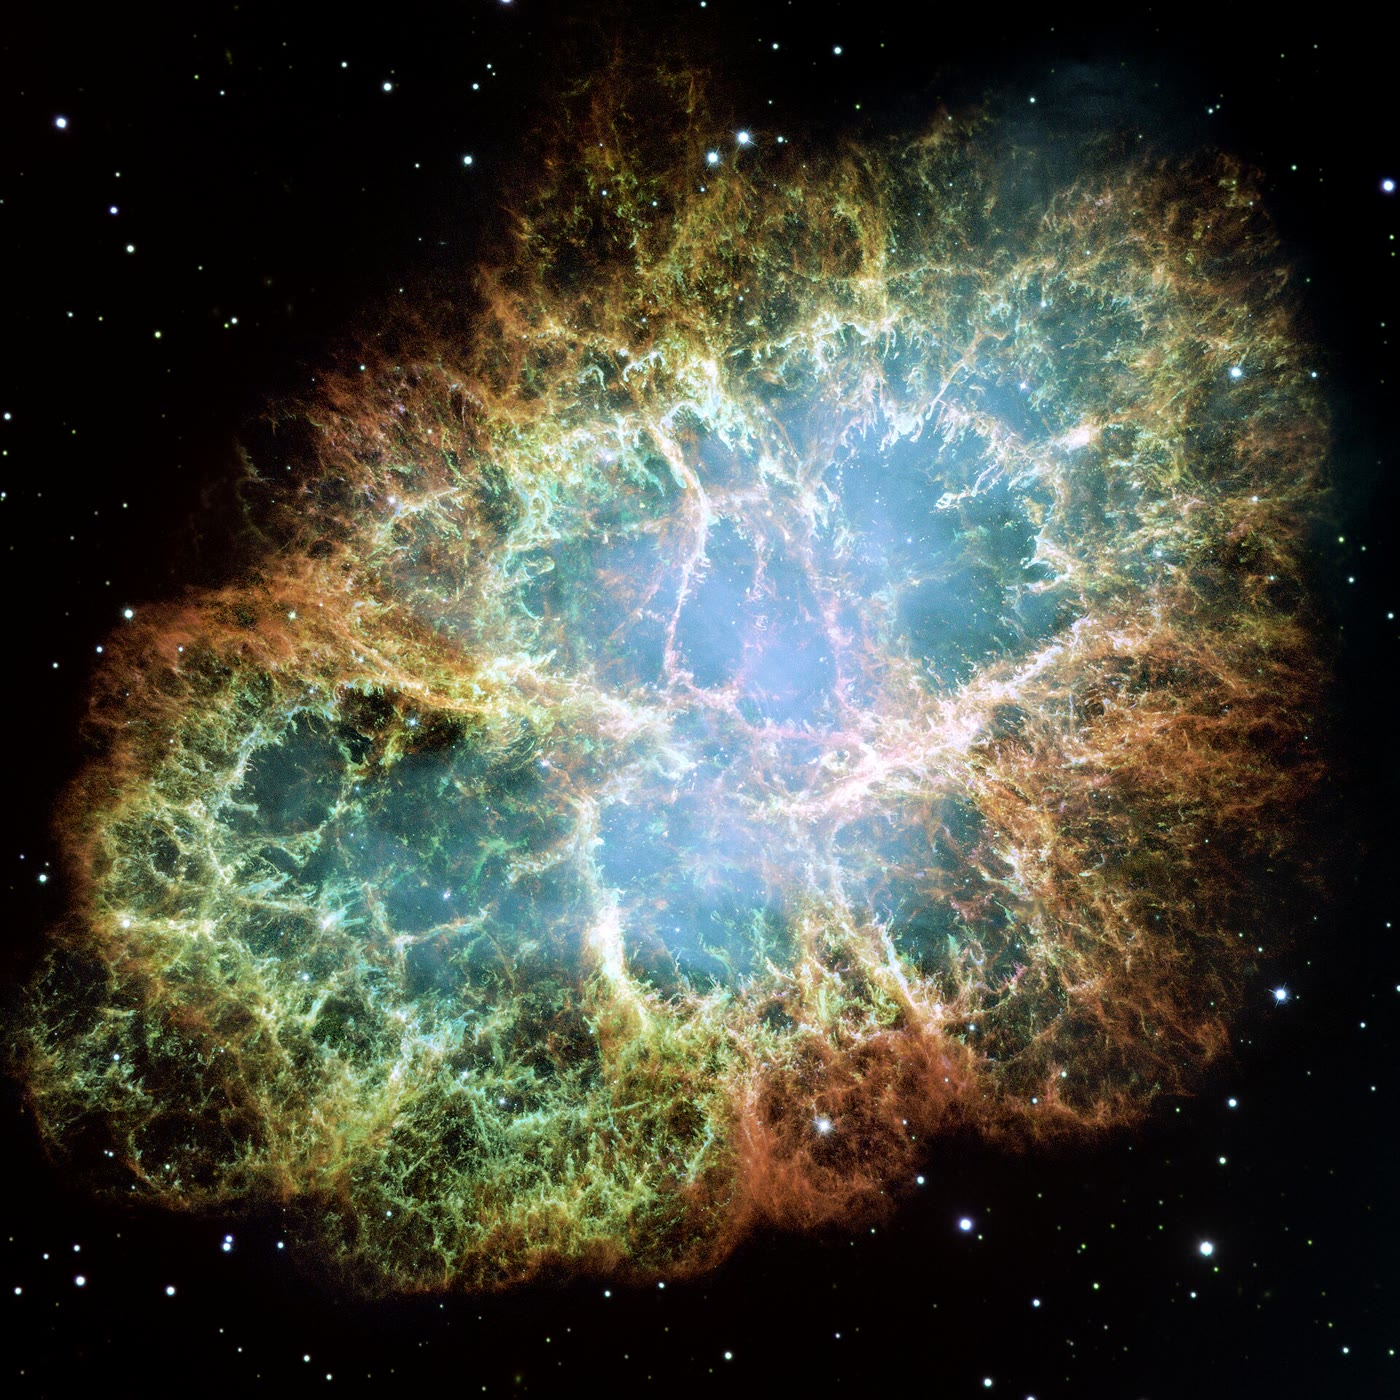
\includegraphics[width=0.5\linewidth]{images/book5/b3-crab-nebula.jpg}
\par\smallskip{\small La Nebulosa del Cangrejo, un mosaico de 24 exposiciones del Telescopio Espacial
Hubble: los restos en expansión de una estrella cuya explosión
registraron astrónomos japoneses y chinos en 1054. Los filamentos anaranjados
son las capas externas deshilachadas de la estrella, sobre todo hidrógeno; el resplandor azulado
del interior procede de electrones que giran en espiral alrededor de las líneas
del campo magnético de la estrella de neutrones central, que gira treinta veces por
segundo. El gas de los filamentos, que transporta lo que formó la estrella, se mezcla
con el medio interestelar. NASA, ESA, J.~Hester y A.~Loll, dominio
público.}\label{fig:b3:origin-of-elements:crab}
\end{omfigure}
% ledger: photo:b3-crab-nebula

\section{Capturas de neutrones}\label{sec:b3:origin-of-elements:neutrons}

Un neutrón no tiene carga eléctrica y no es repelido por un núcleo: incluso
un neutrón lento penetra en él, y el núcleo, una unidad de masa más pesado, libera
la energía de enlace en forma de rayo gamma. Las capturas repetidas originan isótopos más pesados
del mismo elemento hasta que uno resulta inestable; entonces se desintegra,
normalmente por desintegración beta menos, en el elemento siguiente, que a su vez captura
neutrones. Qué núcleos se forman depende de una comparación: el tiempo entre
dos capturas frente a la vida media de los núcleos inestables que se encuentran en el
camino.

\begin{definition}[Captura de neutrones; proceso s; proceso r]\label{def:b3:origin-of-elements:s-process}
La \emph{captura de neutrones}\index{captura de neutrones} es la absorción de un
neutrón libre por un núcleo, $(Z, A) + \mathrm{n} \to (Z, A+1) + \gamma$.
En el \emph{proceso s}\index{proceso s@proceso s} (lento), las capturas
son más lentas que la mayoría de las desintegraciones beta: el tiempo entre dos capturas sobre un mismo
núcleo es de cientos a miles de años, de modo que un núcleo inestable
casi siempre se desintegra antes de poder capturar, y la cadena de capturas
y desintegraciones sigue el valle de estabilidad. En el
\emph{proceso r}\index{proceso r@proceso r} (rápido), la densidad de neutrones
es tan alta que las capturas son mucho más rápidas que las desintegraciones: los núcleos son
llevados a isótopos muy ricos en neutrones, lejos de la estabilidad, en unos pocos
segundos, y se desintegran de vuelta a la estabilidad cuando se agotan los neutrones.
\end{definition}
% ledger: cowan21:timescales, cowan21:rprocess, kaeppeler11:overview

Los dos procesos alcanzan núcleos distintos, y la carta de nucleídos
muestra cuáles. La figura siguiente dibuja una franja de ella, desde el cadmio hasta el
bario. El \omterm{def:b3:origin-of-elements:s-process}{proceso s} la recorre siguiendo el valle de estabilidad: a lo largo de una
fila de un elemento mientras los isótopos son estables, y luego una fila hacia arriba mediante una
desintegración beta. El \omterm{def:b3:origin-of-elements:s-process}{proceso r} procede del lado rico en neutrones, abajo
a la derecha: cada núcleo muy rico en neutrones se desintegra mediante sucesivas desintegraciones beta menos
a lo largo de su isobara, conservando su número másico, y se detiene en el primer
núcleo estable que encuentra. Un núcleo estable que tiene una isobara estable de
menor $Z$ queda \emph{apantallado} frente al \omterm{def:b3:origin-of-elements:s-process}{proceso r}: $^{122}\mathrm{Te}$
queda detrás de $^{122}\mathrm{Sn}$, $^{123}\mathrm{Te}$ detrás de
$^{123}\mathrm{Sb}$, $^{124}\mathrm{Te}$ detrás de $^{124}\mathrm{Sn}$.
Estos tres solo pueden formarse por el \omterm{def:b3:origin-of-elements:s-process}{proceso s}: son
\emph{solo s}. Por el contrario, $^{128}\mathrm{Te}$ y $^{130}\mathrm{Te}$
quedan más allá de la vía s, lo que deja al telurio en $^{127}\mathrm{Te}$,
cuya vida media es \qty{9.35}{h}: son solo r.
% ledger: kaeppeler11:overview, data:b5-iaea-gs, data:b5-sigman

\begin{omfigure}
\centering
\begin{tikzpicture}
\begin{axis}[x=0.62cm, y=0.7cm, xmin=61.4, xmax=84.6, ymin=47.4, ymax=56.6,
  xlabel={número de neutrones $N$}, ylabel={},
  xtick={62,64,...,84}, ytick={48,...,56},
  yticklabels={Cd 48, In 49, Sn 50, Sb 51, Te 52, I 53, Xe 54, Cs 55, Ba 56},
  tick label style={font=\scriptsize}, label style={font=\small},
  axis line style={black!40}, clip=false,
  scatter/classes={0={mark=square*, mark size=6.5pt, blue!45},
    1={mark=square*, mark size=6.5pt, black!18},
    2={mark=square*, mark size=6.5pt, red!40},
    3={mark=square*, mark size=6.5pt, orange!45}}]
\addplot[only marks, mark=square, mark size=6.5pt, black!45, thin,
  restrict x to domain=61:85]
  table[x=N, y=Z] {figdata/out/bachelor-3-neutron_capture-unstable.dat};
\addplot[scatter, only marks, scatter src=explicit symbolic,
  restrict x to domain=61:85]
  table[x=N, y=Z, meta=cls] {figdata/out/bachelor-3-neutron_capture-chart.dat};
\addplot[only marks, mark=none, nodes near coords={\massnum},
  restrict x to domain=61:85,
  visualization depends on={value \thisrow{A} \as \massnum},
  nodes near coords align={center}, every node near coord/.append style={font=\tiny}]
  table[x=N, y=Z] {figdata/out/bachelor-3-neutron_capture-chart.dat};
\addplot[only marks, mark=none, nodes near coords={\massnum}, restrict x to domain=61:85,
  visualization depends on={value \thisrow{A} \as \massnum},
  nodes near coords align={center}, every node near coord/.append style={font=\tiny, black!55}]
  table[x=N, y=Z] {figdata/out/bachelor-3-neutron_capture-unstable.dat};
\addplot[quiver={u=0.48*\thisrow{dN}, v=0.48*\thisrow{dZ}}, -{Stealth[length=3pt]},
  blue!60!black, semithick, restrict x to domain=61:85]
  table[x expr=\thisrow{N0}+0.26*\thisrow{dN}, y expr=\thisrow{Z0}+0.26*\thisrow{dZ}]
  {figdata/out/bachelor-3-neutron_capture-path.dat};
\begin{scope}[red!70!black, dashed, -{Stealth[length=4pt]}, thick]
\draw (axis cs:79.1,48.9) -- (axis cs:76.4,51.6);
\draw (axis cs:81.1,48.9) -- (axis cs:78.4,51.6);
\draw (axis cs:83.1,50.9) -- (axis cs:80.4,53.6);
\end{scope}
\node[font=\scriptsize, red!70!black, anchor=south east, align=right] at (axis cs:84.5,47.5)
  {decaimientos del proceso r\\[-1pt]a lo largo de las isobaras};
\end{axis}
\end{tikzpicture}
\par\smallskip{\small Franja de la carta de nucleídos, desde el cadmio
hasta el bario, números de neutrones de 62 a 84. Los cuadrados coloreados son los núcleos presentes en la naturaleza, marcados
con su número másico: azul, solo s; gris, formados por ambos procesos; rojo,
solo r; naranja, \omterm{def:b3:origin-of-elements:p-process}{núcleos p}, no alcanzados por ninguno. Los cuadrados vacíos son los
núcleos inestables por los que pasa el \omterm{def:b3:origin-of-elements:s-process}{proceso s}. Flechas azules: la vía s,
capturas hacia la derecha, desintegraciones beta en diagonal hacia arriba y a la izquierda (en
$^{134}\mathrm{Cs}$ y $^{135}\mathrm{Cs}$ la vía se bifurca). Flechas rojas discontinuas:
tres de las cadenas de desintegración del \omterm{def:b3:origin-of-elements:s-process}{proceso r}, que terminan en
$^{128}\mathrm{Te}$, $^{130}\mathrm{Te}$ y $^{134}\mathrm{Xe}$. Las
clases se calculan a partir de los isótopos presentes en la naturaleza (Asplund,
Amarsi y Grevesse, 2021) y de las vidas medias y los modos de desintegración de la
carta de nucleídos del OIEA.}\label{fig:b3:origin-of-elements:chart}
\end{omfigure}
% ledger: data:b5-sigman, data:b5-iaea-gs, data:b5-asplund21, kaeppeler11:branchings

Un tercer grupo, los cuadrados naranjas, no lo alcanza ninguno de los dos procesos: los
isótopos ricos en protones, como $^{112}\mathrm{Sn}$, $^{120}\mathrm{Te}$
o $^{124}\mathrm{Xe}$.

\begin{definition}[núcleos p]\label{def:b3:origin-of-elements:p-process}
Los \emph{núcleos p}\index{núcleos p} son los isótopos estables del lado
rico en protones del valle de estabilidad, más allá del pico del hierro, que ni el
\omterm{def:b3:origin-of-elements:s-process}{proceso s} ni el \omterm{def:b3:origin-of-elements:s-process}{proceso r} pueden producir: están protegidos del \omterm{def:b3:origin-of-elements:s-process}{proceso r} por
un isóbaro estable de $Z$ menor y quedan fuera de la trayectoria del \omterm{def:b3:origin-of-elements:s-process}{proceso s}. Se
atribuyen a un proceso p separado, probablemente en explosiones de supernova, y, con
pocas excepciones, sus abundancias son mucho menores que las de los isótopos s y r
vecinos.
\end{definition}
% ledger: kaeppeler11:overview

La regla que lee la carta, aplicada a los 287 nucleidos de la
tabla protosolar más allá del zinc, encuentra 30 núcleos solo-s, 29 núcleos solo-r
y 36 \omterm{def:b3:origin-of-elements:p-process}{núcleos p}. Uno de estos \omterm{def:b3:origin-of-elements:p-process}{núcleos p}, $^{176}\mathrm{Hf}$, en realidad
lo alcanza el \omterm{def:b3:origin-of-elements:s-process}{proceso s} a través de un estado excitado de larga vida del
$^{176}\mathrm{Lu}$ que la regla simple ignora; los otros 35 son los \omterm{def:b3:origin-of-elements:p-process}{núcleos p}
de la literatura.
% ledger: data:b5-sigman, kaeppeler11:branchings

El \omterm{def:b3:origin-of-elements:s-process}{proceso s} puede seguirse cuantitativamente, porque sus núcleos están cerca
de la estabilidad y sus secciones eficaces de captura pueden medirse. En un plasma estelar
a temperatura $T$ los neutrones están termalizados, y lo que importa es la
sección eficaz promediada sobre su distribución de Maxwell--Boltzmann,
$\langle\sigma\rangle$, que se da para una energía térmica
$kT = \qty{30}{keV}$.
% ledger: kaeppeler11:classical

\begin{proposition}[La relación $\sigma N$]\label{prop:b3:origin-of-elements:sigma-n}
\index{relación sigma N@relación $\sigma N$}
En un tramo de la trayectoria s donde todos los núcleos son estables y la
densidad de neutrones $n_\mathrm{n}$ y la temperatura son constantes, sea $N_A$ la
abundancia del núcleo de número másico $A$ y $\langle\sigma\rangle_A$ su
sección eficaz promediada. Si el flujo de neutrones ha alcanzado un
estado estacionario, entonces
\[
\langle\sigma\rangle_{A-1} N_{A-1} = \langle\sigma\rangle_A N_A ,
\]
de modo que el producto $\sigma N$ es el mismo para todos los núcleos del
tramo.
\end{proposition}

\begin{proof}
Un núcleo de masa $A$ captura neutrones a razón de
$\lambda_A = n_\mathrm{n}\langle\sigma\rangle_A v_T$ por núcleo, siendo
$v_T$ la velocidad térmica media de los neutrones. Se forma por capturas sobre
$A - 1$ y se destruye por capturas sobre sí mismo, de modo que
$\mathrm{d}N_A/\mathrm{d}t = n_\mathrm{n} v_T\,(\langle\sigma\rangle_{A-1}
N_{A-1} - \langle\sigma\rangle_A N_A)$. En un estado estacionario la derivada
se anula, y eso es la relación. Un núcleo con una sección eficaz grande
se transforma rápidamente en otro y se mantiene raro; uno con una sección eficaz pequeña
se acumula.
\end{proof}
% ledger: kaeppeler11:classical

Los tres isótopos solo-s del telurio lo ponen a prueba. Sus
abundancias protosolares son \num{0.1067}, \num{0.0373} y \num{0.1984} átomos por
cada millón de átomos de silicio, y sus secciones eficaces \num{295}, \num{832} y
\qty{155}{mb}: los productos son \num{31.5}, \num{31.0} y
\qty{30.8}{mb}, iguales con un margen del tres por ciento, aunque las abundancias
difieren en un factor de cinco. Al cruzar un número mágico de neutrones la
relación se rompe: los núcleos con $N = 50$, $82$ o $126$ están tan fuertemente ligados que
capturan mal, $\langle\sigma\rangle = \qty{4.0}{mb}$ para
$^{138}\mathrm{Ba}$ frente a \qty{61.2}{mb} para $^{136}\mathrm{Ba}$, y
actúan como cuellos de botella. La figura siguiente muestra el producto para todos los
núcleos solo-s: mesetas planas separadas por escalones cerca de $A = 88$, $140$
y $208$.
% ledger: data:b5-sigman, data:b5-kadonis, kaeppeler11:classical

\begin{omfigure}
\centering
\begin{tikzpicture}
\begin{axis}[width=0.95\linewidth, height=7.4cm, xmin=60, xmax=212,
  ymode=log, ymin=1, ymax=5000, xlabel={número másico $A$},
  ylabel={$\langle\sigma\rangle N$ (mb, por $10^6$ átomos de Si)},
  tick label style={font=\scriptsize}, label style={font=\small},
  legend style={font=\scriptsize, at={(0.5,-0.17)}, anchor=north,
    legend columns=2, draw=none, cells={anchor=west},
    /tikz/every even column/.append style={column sep=1em}}]
\draw[black!35, dotted, thick] (axis cs:88,1) -- (axis cs:88,5000);
\draw[black!35, dotted, thick] (axis cs:139,1) -- (axis cs:139,5000);
\draw[black!35, dotted, thick] (axis cs:208,1) -- (axis cs:208,5000);
\addplot[blue!70!black, thick, const plot]
  table[x=A, y=sigN_model] {figdata/out/bachelor-3-neutron_capture-fitted.dat};
\addlegendentry{modelo clásico ajustado para $A > 90$}
\addplot[only marks, mark=*, mark size=1.7pt, red!70!black]
  table[x=A, y=sigN] {figdata/out/bachelor-3-neutron_capture-sigman.dat};
\addlegendentry{núcleos solo-s}
\begin{scope}[font=\scriptsize]
\node[anchor=south west] at (axis cs:88.5,1.1) {$N = 50$};
\node[anchor=south west] at (axis cs:139.5,1.1) {$N = 82$};
\node[anchor=south east] at (axis cs:207.5,1.1) {$N = 126$};
\node[anchor=south] at (axis cs:123,38) {Te};
\node[anchor=south] at (axis cs:135,33) {Ba};
\node[anchor=north] at (axis cs:149,6.6) {Sm};
\node[anchor=west] at (axis cs:177,1.79) {Lu};
\node[anchor=west] at (axis cs:71,2326) {Ge};
\node[anchor=west] at (axis cs:83,428) {Kr};
\end{scope}
\end{axis}
\end{tikzpicture}
\par\smallskip{\small El producto de la sección eficaz de \omterm{def:b3:origin-of-elements:s-process}{captura de neutrones}
a \qty{30}{keV} (KADoNiS) y la abundancia protosolar (Asplund,
Amarsi y Grevesse, 2021) para los 30 núcleos solo-s. Entre los números mágicos
de neutrones (líneas punteadas) es casi constante; en cada uno el flujo
se estrangula y el producto cae. La línea es el modelo clásico
del \omterm{def:b3:origin-of-elements:s-process}{proceso s} ajustado aquí a los núcleos más pesados que $A = 90$. Los
más ligeros necesitan una segunda componente, más débil, producida en estrellas
masivas.}\label{fig:b3:origin-of-elements:sigma-n}
\end{omfigure}
% ledger: data:b5-sigman, data:b5-kadonis, data:b5-asplund21, kaeppeler11:classical

La línea de la figura es el modelo clásico del \omterm{def:b3:origin-of-elements:s-process}{proceso s}: una pequeña
fracción $G$ del hierro-56 se expone a neutrones, con exposiciones distribuidas
exponencialmente alrededor de un valor medio $\tau_0$, y el flujo se sigue núcleo a núcleo
con las secciones eficaces medidas. Su ajuste a 22 núcleos solo-s
más pesados que $A = 90$ (sin contar el $^{176}\mathrm{Lu}$, que
se desintegra, y el $^{187}\mathrm{Os}$, alimentado por la desintegración del
$^{187}\mathrm{Re}$) da $\tau_0 = \qty{0.31}{mb^{-1}}$ y
$G = \qty{0.054}{\percent}$ del hierro-56 solar, cercano al
\qty{0.04}{\percent} de los análisis detallados, en los que cada núcleo
semilla captura por término medio unos quince neutrones. Los núcleos solo-s
más ligeros, germanio-70 y selenio-76, quedan muy por encima de la línea: necesitan
una segunda componente, más débil, producida en estrellas masivas.
% ledger: data:b5-sigman, kaeppeler11:classical

Cuando un núcleo inestable del camino vive aproximadamente lo mismo que el tiempo
entre dos capturas, el flujo se bifurca: una parte se desintegra y otra captura.
Estas \emph{bifurcaciones} se producen en el $^{79}\mathrm{Se}$, $^{85}\mathrm{Kr}$,
$^{134}\mathrm{Cs}$, $^{147}\mathrm{Pm}$ y $^{151}\mathrm{Sm}$, entre
otros. Una bifurcación permite que parte del flujo evite un núcleo: de los dos
isótopos solo-s del samario, el $^{150}\mathrm{Sm}$ recibe todo
el flujo y el $^{148}\mathrm{Sm}$ solo la parte que dio la vuelta a la
bifurcación en la masa 147, y la razón de sus $\sigma N$, \num{0.87},
mide esa proporción. Como la proporción depende de la densidad de neutrones y
de la temperatura, las bifurcaciones son termómetros y densímetros de las
estrellas donde actuó el \omterm{def:b3:origin-of-elements:s-process}{proceso s}.
% ledger: kaeppeler11:branchings, kaeppeler11:pairs, data:b5-sigman

\begin{inthelab}[Medida de una sección eficaz de captura]
Para medir las secciones eficaces promediadas que necesita el \omterm{def:b3:origin-of-elements:s-process}{proceso s},
los físicos reproducen un espectro estelar de neutrones en un acelerador.
Los protones que inciden sobre un blanco de litio producen neutrones mediante la reacción
$^{7}\mathrm{Li}(\mathrm{p},\mathrm{n})^{7}\mathrm{Be}$, cuyo espectro
imita el de un espectro térmico a $kT = \qty{25}{keV}$, cercano a los
\qty{23}{keV} de los destellos de la capa de helio de una gigante roja. La muestra se sitúa
justo contra el blanco, en el flujo más intenso, y tras la
irradiación, los rayos gamma de los núcleos radiactivos recién formados
se cuentan: este método de activación funciona con muestras de menos de un
microgramo. Cuando el producto es estable, los neutrones se envían en pulsos
y se mide su energía por el tiempo de vuelo a lo largo de una trayectoria, y una esfera de
cristales de fluoruro de bario que rodea la muestra registra la cascada de rayos gamma
de cada captura.
\end{inthelab}
% ledger: kaeppeler11:lab

\begin{history}[Tecnecio en gigantes rojas]
En 1952 P.~W.~Merrill halló las líneas del tecnecio en los espectros de
gigantes rojas de tipo espectral S. El tecnecio no tiene ningún isótopo estable; el que
produce el \omterm{def:b3:origin-of-elements:s-process}{proceso s}, $^{99}\mathrm{Tc}$, tiene una vida media de
\num{211000} años, muy inferior a la vida que estas estrellas
habían vivido. El tecnecio tuvo que formarse en el interior de las estrellas, y
hacía poco. Fue la primera prueba directa de que las estrellas producen elementos. En
1957 E.~M. y G.~R.~Burbidge, W.~A.~Fowler y F.~Hoyle, y
de forma independiente A.~G.~W.~Cameron, formularon el modelo clásico del
\omterm{def:b3:origin-of-elements:s-process}{proceso s}.
\end{history}
% ledger: kaeppeler11:overview, data:b5-iaea-gs

El \omterm{def:b3:origin-of-elements:s-process}{proceso r} deja sus propios picos. Su camino discurre cerca de la línea de goteo
de neutrones, el límite más allá del cual un núcleo no puede retener otro neutrón,
y el flujo se detiene en los núcleos con capas de neutrones cerradas, $N = 50$, $82$ y
$126$, hasta que se desintegran beta. Estos puntos de espera acumulan material;
tras las desintegraciones finales hasta la estabilidad, las acumulaciones quedan en números másicos unas pocas
unidades inferiores a los picos del \omterm{def:b3:origin-of-elements:s-process}{proceso s} de los mismos números mágicos, que
están formados por núcleos estables: cerca de $A = 130$ (teluro y xenón) y
$A = 195$ (platino), frente a $A = 138$ y $208$ de los picos s del
bario y del plomo. La curva de abundancias muestra ambos conjuntos de picos, uno junto a
otro. El \omterm{def:b3:origin-of-elements:s-process}{proceso r} produce aproximadamente la mitad de los elementos pesados; el \omterm{def:b3:origin-of-elements:s-process}{proceso s}
la otra mitad.
% ledger: cowan21:rprocess, kaeppeler11:overview, kaeppeler11:classical

\section{Dónde actúan los procesos}\label{sec:b3:origin-of-elements:sites}

El \omterm{def:b3:origin-of-elements:s-process}{proceso s} principal actúa en gigantes rojas de hasta unas tres masas solares, cerca del
final de su vida, como estrellas de la rama asintótica de las gigantes. Entre destellos
de combustión de helio en una capa alrededor de sus núcleos se forma una capa delgada rica en
carbono-13; a unos \qty{9e7}{K} la reacción
$^{13}\mathrm{C}(\alpha,\mathrm{n})^{16}\mathrm{O}$ libera neutrones
durante unos diez mil años, con densidades de $10^6$ a
\qty{e8}{\text{neutrones}.cm^{-3}}. Durante los propios destellos, por encima de
\qty{2.5e8}{K}, la reacción $^{22}\mathrm{Ne}(\alpha,\mathrm{n})^{25}\mathrm{Mg}$
da lugar a una ráfaga de unos pocos años con densidades de hasta \qty{e10}{cm^{-3}}. Los productos
son arrastrados hasta la superficie, donde se observa el tecnecio, y expulsados
por el viento estelar. El \omterm{def:b3:origin-of-elements:s-process}{proceso s} débil, que produce los núcleos solo-s
más ligeros que $A = 90$, actúa en estrellas masivas durante la combustión del helio y
del carbono.
% ledger: kaeppeler11:sources, kaeppeler11:overview

Las supernovas de colapso del núcleo, el final de las estrellas de más de ocho a diez
masas solares, devuelven los \omterm{def:b3:origin-of-elements:alpha}{elementos alfa} y parte del hierro poco después del
nacimiento de las estrellas, porque las estrellas masivas viven poco tiempo. Las supernovas de tipo~Ia,
enanas blancas que explotan en sistemas binarios, devuelven la mayor parte del
hierro, pero solo tras un retardo: la enana blanca debe formarse primero, a partir de una
estrella de menos de ocho masas solares, y después acumular materia de una
compañera hasta alcanzar la masa de Chandrasekhar, de unas
\qty{1.44}{M_\odot}, o fusionarse con una segunda enana blanca. El \omterm{def:b3:origin-of-elements:s-process}{proceso r} necesita un entorno mucho más
extremo.
% ledger: matteucci21:production, matteucci21:time-delay

\begin{definition}[Fusión de estrellas de neutrones; kilonova]\label{def:b3:origin-of-elements:kilonova}
Una \emph{fusión de estrellas de neutrones}\index{fusión de estrellas de neutrones} es la
coalescencia de dos estrellas de neutrones en un sistema binario cerrado, cuya órbita se ha
reducido por la emisión de ondas gravitacionales. Una parte de la materia rica en neutrones
se expulsa. Una \emph{kilonova}\index{kilonova} es el brillo transitorio
de esa eyecta, calentado por la desintegración radiactiva de los núcleos
del \omterm{def:b3:origin-of-elements:s-process}{proceso r} recién formados, que dura unos días.
\end{definition}
% ledger: cowan21:kilonova, ligo17:gw170817

El 17 de agosto de 2017 los detectores de ondas gravitacionales registraron la
espiral de dos estrellas de neutrones, GW170817, a una distancia de unos
\qty{40}{Mpc}: dos cuerpos de \num{1.17} a \qty{1.60}{M_\odot}, que sumaban
\qty{2.74}{M_\odot}. Un destello de rayos gamma llegó \qty{1.7}{s} después de la
fusión. Menos de once horas más tarde, los telescopios hallaron un nuevo punto de
luz en la galaxia NGC~4993 (figura siguiente). Su brillo ultravioleta se apagó
en dos días, y a lo largo de diez días su luz viró al rojo y al infrarrojo.
Los modelos de esa evolución necesitan varias componentes de eyecta, la
más roja, rica en lantánidos, elementos pesados del \omterm{def:b3:origin-of-elements:s-process}{proceso r} cuya densa
maraña de líneas vuelve opaca la eyecta. La masa total expulsada se estima en
\num{0.03} a \qty{0.08}{M_\odot}: la primera prueba directa
de que las fusiones de estrellas de neutrones producen elementos del \omterm{def:b3:origin-of-elements:s-process}{proceso r}.
% ledger: ligo17:gw170817, mma17:kilonova, cowan21:kilonova

\begin{omfigure}
\centering
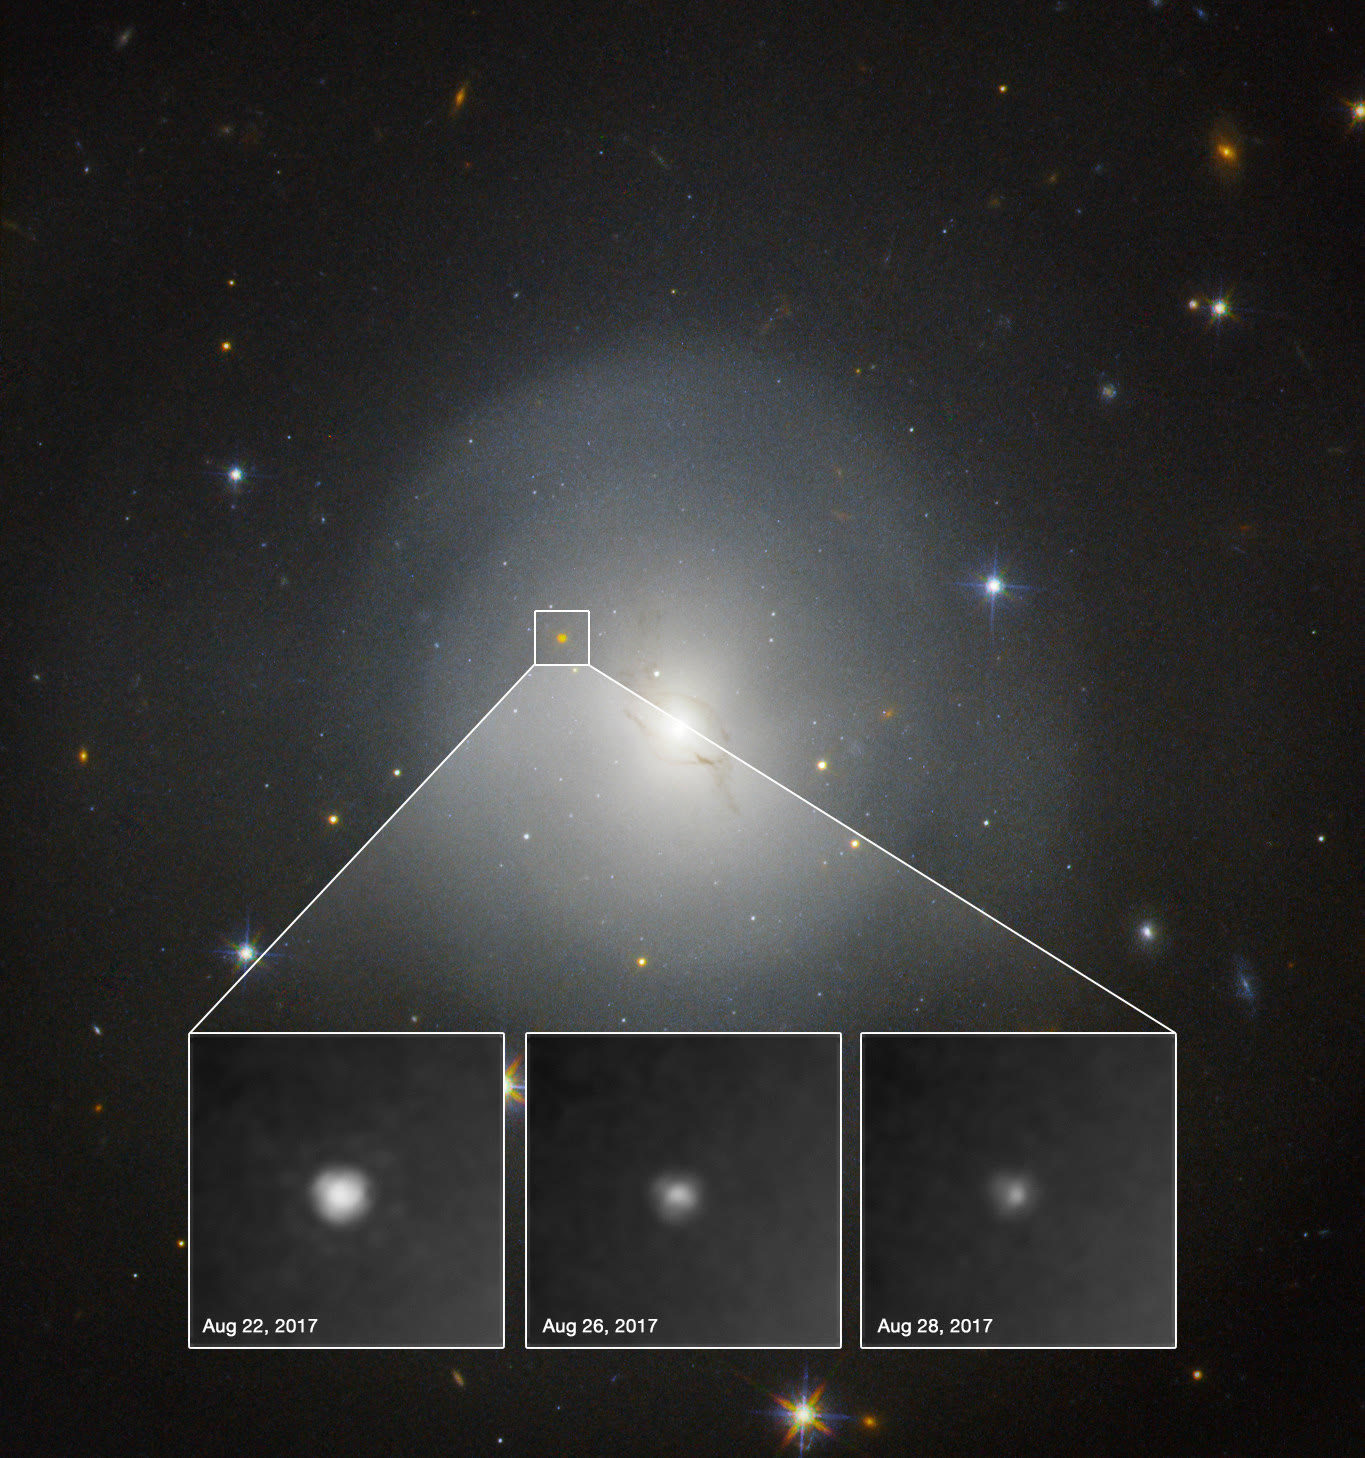
\includegraphics[width=0.55\linewidth]{images/book5/b3-kilonova.jpg}
\par\smallskip{\small La galaxia NGC~4993 fotografiada por el Telescopio Espacial Hubble
tras la fusión de dos estrellas de neutrones detectada en ondas
gravitacionales el 17 de agosto de 2017. El recuadro marca la \omterm{def:b3:origin-of-elements:kilonova}{kilonova}; las
ampliaciones, tomadas el 22, el 26 y el 28 de agosto, la muestran apagándose a lo
largo de seis días. NASA y ESA (A.~J.~Levan, N.~R.~Tanvir, A.~Fruchter y O.~Fox), CC
BY~4.0.}\label{fig:b3:origin-of-elements:kilonova}
\end{omfigure}
% ledger: photo:b3-kilonova

\begin{dated}{2021}
Si las fusiones de estrellas de neutrones producen la mayor parte de los elementos
del \omterm{def:b3:origin-of-elements:s-process}{proceso r} de la Galaxia no está resuelto. Las fusiones deben esperar a que
sus órbitas binarias decaigan, y los modelos de la evolución galáctica en los que
son la única fuente producen los elementos del \omterm{def:b3:origin-of-elements:s-process}{proceso r} demasiado tarde para
explicar lo que se observa en las estrellas más antiguas y más pobres en metales.
Otros candidatos son los tipos raros de supernova de colapso de núcleo, con rotación
rápida y campos magnéticos intensos, y el colapso de estrellas muy masivas; un
modelo de la Galaxia explica el europio observado si alrededor del tres por ciento
de las hipernovas de 25 a \qty{50}{M_\odot} son del tipo impulsado
magnéticamente.
\end{dated}
% ledger: kobayashi20:origins, cowan21:rprocess

\section{La evolución química de la Galaxia}\label{sec:b3:origin-of-elements:gce}

Cada generación de estrellas devuelve al gas parte de lo que fabricó, y la siguiente
generación se forma a partir de ese gas enriquecido. La composición de una estrella
registra, por tanto, la composición del gas en el momento de su nacimiento, y las
estrellas de una galaxia, ordenadas por edad, registran su historia.

\begin{definition}[Evolución química galáctica]\label{def:b3:origin-of-elements:gce}
La \emph{evolución química galáctica}\index{evolución química galáctica}
es el cambio de la composición del gas y de las estrellas de una galaxia con el
tiempo, bajo la acción combinada de la formación estelar, los \omterm{def:b3:origin-of-elements:yield}{rendimientos
estelares}, las vidas de las estrellas y el gas que fluye hacia la galaxia o es
expulsado de ella; y el estudio de ese cambio mediante modelos comparados con las
abundancias de estrellas de edad conocida.
\end{definition}
% ledger: matteucci21:simple

El modelo más sencillo trata una región de una galaxia como una única caja bien
mezclada de gas que se transforma lentamente en estrellas. Sea $s$ la masa retenida
en estrellas de larga vida y en restos estelares, $M_\mathrm{g}$ la masa de gas y
$M = M_\mathrm{g} + s$ la total. El \emph{rendimiento por generación estelar} $y$ es
la masa de metales nuevos que una generación de estrellas devuelve al gas por unidad
de masa que retiene.
% ledger: matteucci21:yield

\begin{theorem}[Modelo de caja cerrada]\label{thm:b3:origin-of-elements:closed-box}
\index{modelo de caja cerrada}
Considérese una región que no intercambia gas con su entorno, que parte de gas puro
sin metales, que permanece bien mezclada y en la que las estrellas que fabrican
metales mueren de inmediato mientras las demás viven para siempre (reciclaje
instantáneo). Entonces la \omterm{def:b3:origin-of-elements:metallicity}{metalicidad} del gas es
\[
Z = y \ln\frac{1}{\mu}, \qquad \mu = \frac{M_\mathrm{g}}{M},
\]
donde $\mu$ es la fracción de gas, y la masa de estrellas formadas con una
\omterm{def:b3:origin-of-elements:metallicity}{metalicidad} inferior a $Z$ es \mbox{$M\,(1 - \mathrm{e}^{-Z/y})$}.
\end{theorem}

\begin{proof}
Cuando una masa $\mathrm{d}s$ queda encerrada en estrellas, el gas pierde
$\mathrm{d}s$, junto con los metales que contiene, $Z\,\mathrm{d}s$,
y gana $y\,\mathrm{d}s$ de metales nuevos:
$\mathrm{d}M_\mathrm{g} = -\mathrm{d}s$ y
$\mathrm{d}(Z M_\mathrm{g}) = (y - Z)\,\mathrm{d}s$. Desarrollando la
segunda, $M_\mathrm{g}\,\mathrm{d}Z + Z\,\mathrm{d}M_\mathrm{g} =
y\,\mathrm{d}s - Z\,\mathrm{d}s$, y los términos en $Z$ se cancelan:
$M_\mathrm{g}\,\mathrm{d}Z = -y\,\mathrm{d}M_\mathrm{g}$. Integrando desde
$M_\mathrm{g} = M$, $Z = 0$ se obtiene $Z = y\ln(M/M_\mathrm{g})$. Las
estrellas formadas mientras la \omterm{def:b3:origin-of-elements:metallicity}{metalicidad} del gas era inferior a $Z$ son las formadas
mientras el gas pasaba de $M$ a $M\mathrm{e}^{-Z/y}$, una masa
$M(1 - \mathrm{e}^{-Z/y})$.
\end{proof}
% ledger: matteucci21:simple

El modelo predice la distribución de \omterm{def:b3:origin-of-elements:metallicity}{metalicidades} de las estrellas de larga vida.
En el vecindario solar la densidad superficial de gas es
\qty{13.7}{M_\odot.pc^{-2}} y la de estrellas y restos estelares
\qty{33.4}{M_\odot.pc^{-2}}, así que $\mu = 13.7/47.1 = 0.29$. Si el gas actual
tiene la $Z = 0.0154$ protosolar, el rendimiento es
$y = 0.0154/\ln(1/0.29) = 0.0125$, y la fracción de todas las estrellas formadas
hasta ahora que tienen $Z$ por debajo de una décima parte del valor actual,
$[\mathrm{Fe/H}] < -1$ si el hierro sigue a los metales, es
$(1 - 0.29^{0.1})/(1 - 0.29) = 0.16$.
% ledger: mckee15:surface, asplund21:xyz, data:b5-gce

\begin{omfigure}
\centering
\begin{tikzpicture}
\begin{axis}[width=0.95\linewidth, height=7.2cm, xmin=-1.6, xmax=0.7,
  ymin=0, ymax=1500, xlabel={$[\mathrm{Fe/H}]$},
  ylabel={número de estrellas por \num{0.1}~dex},
  tick label style={font=\scriptsize}, label style={font=\small},
  legend style={font=\scriptsize, at={(0.5,-0.17)}, anchor=north,
    legend columns=3, draw=none, cells={anchor=west},
    /tikz/every even column/.append style={column sep=1em}}]
\addplot[ybar, area legend, bar width=0.085, fill=black!25, draw=black!50, bar shift=0pt]
  table[x=feh, y=n_obs] {figdata/out/bachelor-3-chemical_evolution-mdf.dat};
\addlegendentry{enanas F y G (6670)}
\addplot[ybar, area legend, bar width=0.085, fill=blue!55, draw=blue!70!black, bar shift=0pt]
  table[x=feh, y=n_low] {figdata/out/bachelor-3-chemical_evolution-mdf.dat};
\addlegendentry{como máximo \qty{1}{M_\odot} (902)}
\addplot[red!75!black, very thick, const plot mark mid]
  table[x=feh, y=model] {figdata/out/bachelor-3-chemical_evolution-mdf.dat};
\addlegendentry{caja cerrada}
\draw[black!50, dashed] (axis cs:-1,0) -- (axis cs:-1,1500);
\node[font=\scriptsize, anchor=north west, align=left] at (axis cs:-1.57,1450)
  {caja cerrada: \qty{16}{\percent}\\por debajo de $-1$;\\observadas: \qty{0.4}{\percent}};
\end{axis}
\end{tikzpicture}
\par\smallskip{\small El \omterm{def:b3:origin-of-elements:g-dwarf}{problema de las enanas G}. Barras: las \omterm{def:b3:origin-of-elements:metallicity}{metalicidades} de
las enanas F y G del vecindario solar (Geneva--Copenhagen,
survey, muestra de mejor fotometría reanalizada por Casagrande y otros,
2011), todas las estrellas en gris, y las de como máximo una masa solar, las
estrellas de larga vida que cuenta el modelo, en azul. Línea: la caja cerrada
con la fracción de gas actual del vecindario solar, escalada al
mismo número de estrellas; no produce ninguna estrella más rica que su
gas actual, tomado como solar. La caja predice una larga cola de estrellas pobres en
metales que no existe.}\label{fig:b3:origin-of-elements:g-dwarf}
\end{omfigure}
% ledger: data:b5-gcs, casagrande11:gcs, data:b5-gce, mckee15:surface

\begin{definition}[Problema de las enanas G]\label{def:b3:origin-of-elements:g-dwarf}
El \emph{problema de las enanas G}\index{problema de las enanas G} es la escasez de
estrellas de vida larga pobres en metales en el vecindario solar, en comparación con la
predicción del \omterm{thm:b3:origin-of-elements:closed-box}{modelo de caja cerrada}: son mucho menos frecuentes las enanas de tipo
espectral G de vida larga con \omterm{def:b3:origin-of-elements:metallicity}{metalicidades} bajas que las que una caja cerrada habría
producido.
\end{definition}
% ledger: matteucci21:simple

De las 6670 estrellas de la muestra del sondeo, 26 tienen $[\mathrm{Fe/H}] < -1$:
\qty{0.4}{\percent}, frente al \qty{16}{\percent} de la caja cerrada.
Incluso entre las 902 estrellas de masa no superior a una masa solar, la comparación más
justa, las 26 representan el \qty{2.9}{\percent}. La salida consiste en abrir la
caja: si el disco del vecindario solar se construyó mediante una acreción lenta
de gas pobre en metales a lo largo de varios miles de millones de años, el gas primitivo nunca fue
un gran reservorio dispuesto a formar estrellas pobres en metales, y la cola
desaparece. Los modelos del disco que reproducen la distribución necesitan un tiempo
de acreción superior a tres o cuatro mil millones de años.
% ledger: data:b5-gcs, data:b5-gce, matteucci21:simple

El segundo reloj es la razón entre dos tipos de elementos. Los \omterm{def:b3:origin-of-elements:alpha}{elementos alfa}
proceden de las supernovas de colapso del núcleo, poco después del nacimiento de una
generación estelar; buena parte del hierro procede de supernovas de tipo Ia,
mucho más tarde. En las estrellas viejas del halo, con $[\mathrm{Fe/H}] < -1$,
$[\alpha/\mathrm{Fe}]$ es de aproximadamente $+0.4$: estas estrellas se formaron a partir de gas
enriquecido solo por supernovas de colapso del núcleo. En las estrellas del disco
disminuye al aumentar la \omterm{def:b3:origin-of-elements:metallicity}{metalicidad} hasta cero, el valor solar, a medida que las
supernovas de tipo Ia aportan su hierro. La figura siguiente muestra el modelo más
sencillo de este esquema de \emph{retardo temporal}: en una caja cerrada, ambos tipos de
supernova empiezan a la vez, salvo que las de tipo Ia comienzan un tiempo fijo después de
las primeras estrellas.
% ledger: matteucci21:time-delay, matteucci21:production

\begin{omfigure}
\centering
\begin{tikzpicture}
\begin{axis}[width=0.8\linewidth, height=6.4cm, xmin=-2.4, xmax=0.25,
  ymin=-0.08, ymax=0.55, xlabel={$[\mathrm{Fe/H}]$},
  ylabel={$[\alpha/\mathrm{Fe}]$},
  tick label style={font=\scriptsize}, label style={font=\small}]
\addplot[black!40, dashed, domain=-2.4:0.25, samples=2] {0};
\addplot[blue!70!black, very thick]
  table[x=feh, y=afe] {figdata/out/bachelor-3-chemical_evolution-alpha.dat};
\addplot[only marks, mark=*, mark size=2pt, red!70!black] coordinates {(-1,0.4) (0,0)};
\node[font=\scriptsize, anchor=south, align=center] at (axis cs:-1.75,0.41)
  {supernovas de colapso del núcleo únicamente};
\node[font=\scriptsize, anchor=south west, align=left] at (axis cs:-0.98,0.41)
  {supernovas de tipo Ia\\[-1pt]comienzan};
\node[font=\scriptsize, anchor=south west] at (axis cs:0.01,0.01) {Sol};
\end{axis}
\end{tikzpicture}
\par\smallskip{\small Modelo de dos fases de $[\alpha/\mathrm{Fe}]$ en una
caja cerrada: la meseta en $+0.4$ es la razón producida por las supernovas de colapso
del núcleo; las supernovas de tipo Ia, que comienzan cuando el gas ha alcanzado
$[\mathrm{Fe/H}] = -1$, luego añaden hierro a ritmo constante, hasta que la razón
es solar en $[\mathrm{Fe/H}] = 0$. La meseta y el codo son los que se observan
en las estrellas de la Galaxia; la forma intermedia es la del modelo.
A la \omterm{def:b3:origin-of-elements:metallicity}{metalicidad} del Sol, el \qty{60}{\percent} del hierro de este modelo
procede de supernovas de tipo Ia.}\label{fig:b3:origin-of-elements:alpha}
\end{omfigure}
% ledger: data:b5-gce, matteucci21:time-delay

Los modelos detallados de la Galaxia que reproducen la tendencia observada
atribuyen dos tercios del hierro a supernovas de tipo Ia y un tercio a
supernovas de colapso del núcleo, y concluyen que el gas de la Galaxia joven
alcanzó $[\mathrm{Fe/H}] = -1$ en unos mil a mil quinientos millones de
años. La razón es un reloj: una población rica en \omterm{def:b3:origin-of-elements:alpha}{elementos alfa} a una \omterm{def:b3:origin-of-elements:metallicity}{metalicidad} dada
formó sus estrellas deprisa, antes de que las supernovas de tipo Ia pudieran aportar
su hierro. El \omterm{def:b3:milky-way-galaxies:structure}{disco grueso} del capítulo anterior es una población de este tipo: antigua,
y levemente enriquecida en \omterm{def:b3:origin-of-elements:alpha}{elementos alfa} en comparación con las estrellas del disco
delgado de la misma \omterm{def:b3:origin-of-elements:metallicity}{metalicidad}.
% ledger: matteucci21:time-delay, casagrande11:gcs

\section{De las abundancias solares a la Tierra}\label{sec:b3:origin-of-elements:earth}

La Tierra está hecha del mismo material que el Sol, pero no de todo él. En la nebulosa
en enfriamiento, solo los elementos que condensaron en sólidos pudieron agruparse en
planetesimales; el volumen de segundo año siguió la secuencia en que condensan.
El hierro condensa como metal aproximadamente a la misma temperatura que los silicatos
de magnesio, de \qtyrange{1310}{1340}{K} a \qty{e-4}{bar}, de modo que los planetas
rocosos conservaron su parte de hierro, mientras que el hidrógeno, el helio, el carbono,
el nitrógeno y los gases nobles permanecieron en el gas.
De un gas de composición solar, solo cerca de un medio por ciento de la masa
condensa como roca y metal.
% ledger: lodders:tc-table, lodders:condensates

\begin{definition}[Tendencia de volatilidad]\label{def:b3:origin-of-elements:volatility}
La \emph{tendencia de volatilidad}\index{tendencia de volatilidad} de un cuerpo planetario
es la disminución de sus abundancias, relativas a las condritas CI y
normalizadas a un elemento refractario, al disminuir la temperatura de condensación:
los elementos refractarios se mantienen en sus proporciones condríticas,
mientras que los moderadamente volátiles se empobrecen tanto más cuanto menor
es su temperatura de condensación.
\end{definition}

Para la Tierra silicática, el volumen de segundo año trazó la tendencia frente a la
temperatura de condensación. Normalizado al magnesio, el circonio (que condensa a
\qty{1741}{K}) se sitúa en \num{1.11} veces su proporción CI, el sodio
(\qty{958}{K}) en \num{0.22}, el potasio (\qty{1006}{K}) en \num{0.19},
el rubidio (\qty{800}{K}) en \num{0.12} y el zinc (\qty{726}{K}) en \num{0.075}.
La Tierra se formó a partir de material que ya había perdido parte de sus elementos
moderadamente volátiles antes de que el planeta se ensamblara, o los perdió durante
su crecimiento. Incluso las condritas CI difieren del Sol de un modo que sigue
la temperatura de condensación, aunque de forma tenue: sus elementos
moderadamente volátiles están unos \num{0.04}~\omterm{def:b3:origin-of-elements:abundance}{dex} por encima de los valores
fotosféricos.
% ledger: lodders:tc-table, lodders:ci-table, ms95:pm-trace, asplund21:abstract

Así, el registro de este capítulo recorre el planeta. El oxígeno, el
magnesio y el silicio del manto son \omterm{def:b3:origin-of-elements:alpha}{elementos alfa} de estrellas masivas; el hierro del
núcleo procede en su mayor parte de supernovas de tipo Ia; el torio y el uranio, cuya
desintegración ayuda a calentar el interior, están más allá del bismuto, donde solo llega
el \omterm{def:b3:origin-of-elements:s-process}{proceso r}; y toda la mezcla
se ordenó por volatilidad antes de que la Tierra la acumulara.
% ledger: matteucci21:production, matteucci21:time-delay, kaeppeler11:overview, data:b5-sigman

\section{Ejercicios}

\begin{exercise}[$\star$]\label{exo:b3:origin-of-elements:1}
Usando las \omterm{def:b3:origin-of-elements:abundance}{abundancias solares} $\log\varepsilon(\mathrm{O}) = 8.69$,
$\log\varepsilon(\mathrm{Si}) = 7.51$, $\log\varepsilon(\mathrm{Fe}) =
7.46$, $\log\varepsilon(\mathrm{Au}) = 0.91$ y
$\log\varepsilon(\mathrm{Pb}) = 1.95$: (a)~¿Cuántos átomos de silicio y
cuántos átomos de oxígeno hay en el Sol por átomo de hierro? (b)~¿Cuántos
átomos de hierro hay por átomo de oro, y cuántos de plomo por átomo de oro?
\end{exercise}

\begin{exercise}[$\star$]\label{exo:b3:origin-of-elements:2}
(a)~¿Cuántos átomos de hierro por millón de átomos de hidrógeno tiene el Sol
($\log\varepsilon(\mathrm{Fe}) = 7.46$)? (b)~Una estrella del halo tiene
$[\mathrm{Fe/H}] = -2$. ¿Cuántos átomos de hidrógeno tiene por
átomo de hierro? (c)~Otra estrella tiene un átomo de hierro por cada diez millones
de átomos de hidrógeno. ¿Cuál es su $[\mathrm{Fe/H}]$?
\end{exercise}

\begin{exercise}[$\star$]\label{exo:b3:origin-of-elements:3}
Los isótopos estables del xenón tienen números másicos 124, 126, 128, 129, 130,
131, 132, 134 y 136. Entre sus isóbaros, el teluro ($Z = 52$) tiene
isótopos estables 120, 122--126, 128 y 130; el yodo ($Z = 53$) solo el 127.
La vía s alcanza el xenón en $^{128}\mathrm{Xe}$, por la desintegración del
$^{128}\mathrm{I}$, y lo abandona en $^{133}\mathrm{Xe}$, que se desintegra.
Clasifíquese cada isótopo del xenón como solo s, solo r, producido por ambos procesos o
núcleo p.
\end{exercise}

\begin{exercise}[$\star$]\label{exo:b3:origin-of-elements:4}
GW170817 se halla a unos \qty{40}{Mpc}, y sus rayos gamma llegaron
\qty{1.7}{s} después de la fusión observada en ondas gravitacionales. (a)~¿Cuánto tiempo
habían viajado ambas señales? (b)~Si el retraso se atribuye por completo a
una diferencia de velocidades entre las dos, ¿cuán grande es esa diferencia como
fracción de la velocidad de la luz, como máximo?
\end{exercise}

\begin{exercise}[$\star\star$]\label{exo:b3:origin-of-elements:5}
Los tres isótopos del teluro de solo \omterm{def:b3:origin-of-elements:s-process}{proceso s} tienen abundancias protosolares
\num{0.1067}, \num{0.0373} y \num{0.1984} por cada $10^6$ átomos de silicio
($A = 122$, $123$, $124$) y secciones eficaces promediadas \num{295},
\num{832} y \qty{155}{mb}. (a)~Calcúlese $\sigma N$ para cada uno. (b)~A partir de
$^{122}\mathrm{Te}$ solamente, estímense las abundancias de $^{123}\mathrm{Te}$
y $^{124}\mathrm{Te}$, y compárense. (c)~¿Por qué no puede aplicarse la relación
a $^{128}\mathrm{Te}$?
\end{exercise}

\begin{exercise}[$\star\star$]\label{exo:b3:origin-of-elements:6}
En el modelo clásico, cada núcleo de la vía s transmite al
siguiente una fracción $f = 1/(1 + 1/(\tau_0\langle\sigma\rangle))$ del
flujo, con $\tau_0 = \qty{0.306}{mb^{-1}}$. (a)~Calcúlese $f$ para
$^{124}\mathrm{Te}$ (\qty{155}{mb}) y para el de número mágico de neutrones,
$^{138}\mathrm{Ba}$ (\qty{4.0}{mb}). (b)~Los núcleos desde
$^{137}\mathrm{Ba}$ hasta $^{142}\mathrm{Nd}$ de la vía tienen
secciones eficaces \num{76.3}, \num{4.0}, \num{32.4}, \num{11.0},
\num{111.4} y \qty{35.0}{mb}. ¿En qué factor disminuye $\sigma N$ desde
$^{136}\mathrm{Ba}$ hasta $^{142}\mathrm{Nd}$? (c)~Compárese con los
valores medidos, \num{27.6} y \qty{7.72}{mb}.
\end{exercise}

\begin{exercise}[$\star\star$]\label{exo:b3:origin-of-elements:7}
Un neutrón de energía térmica $kT$ tiene la velocidad
$v_T = \sqrt{2kT/m_\mathrm{n}}$, $m_\mathrm{n} = \qty{1.6749e-27}{kg}$.
(a)~Calcúlese $v_T$ para $kT = \qty{8}{keV}$, temperatura de la
capa de carbono-13 de una gigante roja. (b)~Para $^{124}\mathrm{Te}$, con
$\langle\sigma\rangle = \qty{155}{mb}$, calcúlese el tiempo medio entre
dos capturas, $1/(n_\mathrm{n}\langle\sigma\rangle v_T)$, para
$n_\mathrm{n} = 10^6$, $10^8$ y \qty{e10}{cm^{-3}}. (c)~Compárese con
las vidas medias de $^{127}\mathrm{Te}$ (\qty{9.35}{h}) y de
$^{134}\mathrm{Cs}$ (\qty{2.07}{yr}). ¿Cuál de ellos es un punto de ramificación?
\end{exercise}

\begin{exercise}[$\star\star$]\label{exo:b3:origin-of-elements:8}
En el Sol, $\log\varepsilon$ vale \num{6.30} para el calcio, \num{3.14} para
el escandio y \num{4.97} para el titanio; \num{1.38} para el berilio,
\num{2.70} para el boro y \num{8.46} para el carbono. (a)~¿Cuántas veces menos abundante es
el escandio que sus dos vecinos? (b)~¿Cuántas veces menos abundante es
el berilio que el carbono? (c)~¿Qué rasgo de la curva de abundancias ilustra
cada uno, y cuál es su causa?
\end{exercise}

\begin{exercise}[$\star\star$]\label{exo:b3:origin-of-elements:9}
En el modelo de dos fases del capítulo, la meseta
$[\alpha/\mathrm{Fe}] = P$ es la razón producida por las supernovas de colapso del núcleo,
y a $[\mathrm{Fe/H}] = 0$ la razón es solar. (a)~Demuéstrese que la fracción
del hierro solar producido por supernovas de tipo Ia es $1 - 10^{-P}$, y calcúlese
esa fracción para $P = 0.4$. (b)~¿Qué meseta daría los dos tercios de
los modelos detallados? (c)~Una galaxia enana muestra su codo en
$[\mathrm{Fe/H}] = -2$. ¿Qué dice eso sobre su formación estelar?
\end{exercise}

\begin{exercise}[$\star\star\star$]\label{exo:b3:origin-of-elements:10}
Las condritas CI contienen, en partes por millón en masa, \num{95870}
de magnesio, \num{3.96} de circonio, \num{5010} de sodio, \num{530}
de potasio y \num{2.13} de rubidio; la Tierra silicatada contiene
\qty{22.8}{\percent} de magnesio y \num{10.5}, \num{2670}, \num{240}
y \num{0.6} partes por millón de los demás. Sus temperaturas de condensación del 50~por~ciento
son \qty{1336}{K} (Mg), \qty{1741}{K} (Zr),
\qty{958}{K} (Na), \qty{1006}{K} (K) y \qty{800}{K} (Rb). (a)~Para
cada elemento, calcúlese $(X/\mathrm{Mg})_\mathrm{Earth}/(X/\mathrm{Mg})_\mathrm{CI}$.
(b)~Represéntese frente a la temperatura de condensación y descríbase la
tendencia. (c)~¿Por qué se elige el magnesio como referencia?
\end{exercise}

\begin{exercise}[$\star\star\star$]\label{exo:b3:origin-of-elements:11}
Una caja con fugas pierde gas en un viento a un ritmo $\lambda$ veces su ritmo de
formación estelar, y no recibe ninguno. (a)~Demuéstrese que su \omterm{def:b3:origin-of-elements:metallicity}{metalicidad} es
$Z = \frac{y}{1 + \lambda}\ln\frac{M_\mathrm{g}(0)}{M_\mathrm{g}}$.
(b)~Con $y = 0.0125$, compárese la \omterm{def:b3:origin-of-elements:metallicity}{metalicidad} alcanzada cuando el gas se ha
reducido al \qty{29}{\percent} de su masa inicial para $\lambda = 0$ y
$\lambda = 1$. (c)~¿Por qué las galaxias pequeñas, con gravedad débil, tienden a ser
pobres en metales?
\end{exercise}

\begin{exercise}[$\star\star\star$]\label{exo:b3:origin-of-elements:12}
(a)~El Sol tiene $\log\varepsilon(\mathrm{Li}) = 0.96$ en su fotosfera
y las condritas CI $3.25$. Calcúlense las dos razones $N_\mathrm{Li}/N_\mathrm{H}$
y la fracción de su litio que el Sol ha destruido. (b)~Las estrellas más antiguas
pobres en metales muestran $N_\mathrm{Li}/N_\mathrm{H} = \num{1.45e-10}$,
mientras que la nucleosíntesis del Big Bang predice \num{4.72e-10}. ¿En qué factor
supera el litio del Sistema Solar a cada uno de estos valores? (c)~¿Qué implican las dos
comparaciones?
\end{exercise}

\section{Problema: galaxia de caja cerrada}

\begin{problem}[{Problema de fin de semana --- desde la mezcla solar hasta las
metalicidades de las estrellas de larga vida}]
\label{pb:b3:origin-of-elements:1}
Utilícense $\log\varepsilon(\mathrm{H}) = 12$, las \omterm{def:b3:origin-of-elements:abundance}{abundancias solares}
$\log\varepsilon(\mathrm{Fe}) = 7.46$, $\log\varepsilon(\mathrm{O}) =
8.69$, $\log\varepsilon(\mathrm{He}) = 10.914$, las actuales
fracciones de masa fotosféricas $X = 0.7438$, $Y = 0.2423$, $Z = 0.0139$,
y el $Z_\odot = 0.0154$ protosolar. Supóngase en todo momento que el hierro
sigue a la \omterm{def:b3:origin-of-elements:metallicity}{metalicidad} total, $[\mathrm{Fe/H}] = \log_{10}(Z/Z_\odot)$.

\medskip\noindent\textbf{Parte I --- La mezcla solar.}
\begin{enumerate}
\item ¿Cuántos átomos de hidrógeno hay en el Sol por cada átomo de hierro?
\item Calcúlese la razón numérica $N_\mathrm{He}/N_\mathrm{H}$. Tomando un
  átomo de helio cuatro veces más pesado que uno de hidrógeno, compárese
  $4N_\mathrm{He}/N_\mathrm{H}$ con $Y/X$.
\item Una estrella tiene un átomo de hierro por cada \num{350000} átomos de hidrógeno.
  Calcúlese su $[\mathrm{Fe/H}]$ con dos decimales.
\item La misma estrella tiene $[\mathrm{O/Fe}] = +0.40$. Calcúlese su
  $\log\varepsilon(\mathrm{O})$, y su número de átomos de oxígeno por átomo
  de hierro comparado con el del Sol.
\item El oxígeno es el metal más abundante. Estímese la fracción de masa
  metálica de la estrella escalando la del Sol con $[\mathrm{O/H}]$.
\item ¿Por qué la \omterm{def:b3:origin-of-elements:metallicity}{metalicidad} de una estrella se suele medir a partir del hierro
  y no a partir del oxígeno, aunque el oxígeno domine $Z$?
\end{enumerate}

\medskip\noindent\textbf{Parte II --- El proceso s sobre el telurio.} Utilícense
los datos del \cref{exo:b3:origin-of-elements:5}.
\begin{enumerate}[resume]
\item Explíquese a partir de la carta de nucleidos por qué $^{122}\mathrm{Te}$,
  $^{123}\mathrm{Te}$ y $^{124}\mathrm{Te}$ son solo-s.
\item Calcúlese $\sigma N$ para los tres isótopos y su media.
\item Predígase la abundancia de $^{123}\mathrm{Te}$ a partir de la media de los
  otros dos, y déese la diferencia respecto del valor medido, en por
  ciento.
\item $^{128}\mathrm{Te}$ tiene $N = 1.329$ por $10^6$ átomos de Si y
  $\langle\sigma\rangle = \qty{44.4}{mb}$. Calcúlese su $\sigma N$ y
  explíquese por qué no está en la meseta.
\item El par solo-s $^{148}\mathrm{Sm}$ y $^{150}\mathrm{Sm}$ tiene
  $\sigma N = \num{7.43}$ y \qty{8.53}{mb}. ¿Qué fracción del flujo
  pasó por $^{148}\mathrm{Sm}$, y a través de qué ramificación?
\item A lo largo de $N = 82$ el producto cae desde \qty{27.6}{mb}
  ($^{136}\mathrm{Ba}$) hasta \qty{7.72}{mb} ($^{142}\mathrm{Nd}$). ¿Qué
  propiedad de los núcleos con $N = 82$ explica la caída?
\end{enumerate}

\medskip\noindent\textbf{Parte III --- La caja cerrada.} El entorno solar
tiene \qty{13.7}{M_\odot.pc^{-2}} de gas y
\qty{33.4}{M_\odot.pc^{-2}} de estrellas y remanentes estelares. Supóngase que el
gas actual tiene $Z = Z_\odot$.
\begin{enumerate}[resume]
\item Calcúlese la fracción de gas actual $\mu_1$.
\item Calcúlese el rendimiento por generación estelar $y$ que necesita la caja
  cerrada, y su razón respecto a $Z_\odot$.
\item Calcúlense $Z$ y $[\mathrm{Fe/H}]$ del gas cuando la fracción de gas
  era $0.9$, y luego $0.5$.
\item Calcúlese la fracción de gas cuando el gas alcanzó
  $[\mathrm{Fe/H}] = -1$.
\item ¿Qué fracción de la masa total había quedado entonces retenida en estrellas?
\item Si la fracción de gas actual fuera $0.1$, ¿qué rendimiento necesitaría
  la caja?
\end{enumerate}

\medskip\noindent\textbf{Parte IV --- La distribución de metalicidades.}
\begin{enumerate}[resume]
\item Muéstrese que la caja cerrada da una distribución de estrellas en
  $[\mathrm{Fe/H}]$ proporcional a $Z\,\mathrm{e}^{-Z/y}$, y hállese el
  $[\mathrm{Fe/H}]$ de su máximo.
\item Calcúlese la fracción de todas las estrellas formadas hasta el momento con
  $[\mathrm{Fe/H}] < -1$.
\item Calcúlese la fracción con $[\mathrm{Fe/H}] < -0.5$.
\item En la muestra de estudio de 6670 enanas F y G, 26 tienen
  $[\mathrm{Fe/H}] < -1$. ¿Cuántas predice la caja cerrada?
\item Entre las 902 estrellas de masa no superior a una masa solar se encuentran
  las mismas 26. Calcúlese la fracción observada, y explíquese por qué esta
  submuestra es la comparación más justa.
\item Con una fracción de gas actual de $0.1$, ¿cuál sería la fracción predicha
  por debajo de $-1$? ¿Resuelve otra fracción de gas el
  problema?
\item Calcúlese la fracción de estrellas de larga vida con $[\mathrm{Fe/H}] < -1$
  que predice la caja cerrada para el entorno solar, en por ciento, con dos
  cifras significativas, y explíquese qué implica la comparación con las
  estrellas observadas para la historia del disco.
\end{enumerate}
\end{problem}
% ledger: asplund21:abstract, asplund21:xyz, data:b5-sigman, data:b5-kadonis, mckee15:surface, data:b5-gcs, data:b5-gce, matteucci21:simple
